% Options for packages loaded elsewhere
\PassOptionsToPackage{unicode}{hyperref}
\PassOptionsToPackage{hyphens}{url}
%
\documentclass[
]{article}
\usepackage{amsmath,amssymb}
\usepackage{lmodern}
\usepackage{iftex}
\ifPDFTeX
  \usepackage[T1]{fontenc}
  \usepackage[utf8]{inputenc}
  \usepackage{textcomp} % provide euro and other symbols
\else % if luatex or xetex
  \usepackage{unicode-math}
  \defaultfontfeatures{Scale=MatchLowercase}
  \defaultfontfeatures[\rmfamily]{Ligatures=TeX,Scale=1}
\fi
% Use upquote if available, for straight quotes in verbatim environments
\IfFileExists{upquote.sty}{\usepackage{upquote}}{}
\IfFileExists{microtype.sty}{% use microtype if available
  \usepackage[]{microtype}
  \UseMicrotypeSet[protrusion]{basicmath} % disable protrusion for tt fonts
}{}
\makeatletter
\@ifundefined{KOMAClassName}{% if non-KOMA class
  \IfFileExists{parskip.sty}{%
    \usepackage{parskip}
  }{% else
    \setlength{\parindent}{0pt}
    \setlength{\parskip}{6pt plus 2pt minus 1pt}}
}{% if KOMA class
  \KOMAoptions{parskip=half}}
\makeatother
\usepackage{xcolor}
\usepackage[margin=1in]{geometry}
\usepackage{color}
\usepackage{fancyvrb}
\newcommand{\VerbBar}{|}
\newcommand{\VERB}{\Verb[commandchars=\\\{\}]}
\DefineVerbatimEnvironment{Highlighting}{Verbatim}{commandchars=\\\{\}}
% Add ',fontsize=\small' for more characters per line
\usepackage{framed}
\definecolor{shadecolor}{RGB}{248,248,248}
\newenvironment{Shaded}{\begin{snugshade}}{\end{snugshade}}
\newcommand{\AlertTok}[1]{\textcolor[rgb]{0.94,0.16,0.16}{#1}}
\newcommand{\AnnotationTok}[1]{\textcolor[rgb]{0.56,0.35,0.01}{\textbf{\textit{#1}}}}
\newcommand{\AttributeTok}[1]{\textcolor[rgb]{0.77,0.63,0.00}{#1}}
\newcommand{\BaseNTok}[1]{\textcolor[rgb]{0.00,0.00,0.81}{#1}}
\newcommand{\BuiltInTok}[1]{#1}
\newcommand{\CharTok}[1]{\textcolor[rgb]{0.31,0.60,0.02}{#1}}
\newcommand{\CommentTok}[1]{\textcolor[rgb]{0.56,0.35,0.01}{\textit{#1}}}
\newcommand{\CommentVarTok}[1]{\textcolor[rgb]{0.56,0.35,0.01}{\textbf{\textit{#1}}}}
\newcommand{\ConstantTok}[1]{\textcolor[rgb]{0.00,0.00,0.00}{#1}}
\newcommand{\ControlFlowTok}[1]{\textcolor[rgb]{0.13,0.29,0.53}{\textbf{#1}}}
\newcommand{\DataTypeTok}[1]{\textcolor[rgb]{0.13,0.29,0.53}{#1}}
\newcommand{\DecValTok}[1]{\textcolor[rgb]{0.00,0.00,0.81}{#1}}
\newcommand{\DocumentationTok}[1]{\textcolor[rgb]{0.56,0.35,0.01}{\textbf{\textit{#1}}}}
\newcommand{\ErrorTok}[1]{\textcolor[rgb]{0.64,0.00,0.00}{\textbf{#1}}}
\newcommand{\ExtensionTok}[1]{#1}
\newcommand{\FloatTok}[1]{\textcolor[rgb]{0.00,0.00,0.81}{#1}}
\newcommand{\FunctionTok}[1]{\textcolor[rgb]{0.00,0.00,0.00}{#1}}
\newcommand{\ImportTok}[1]{#1}
\newcommand{\InformationTok}[1]{\textcolor[rgb]{0.56,0.35,0.01}{\textbf{\textit{#1}}}}
\newcommand{\KeywordTok}[1]{\textcolor[rgb]{0.13,0.29,0.53}{\textbf{#1}}}
\newcommand{\NormalTok}[1]{#1}
\newcommand{\OperatorTok}[1]{\textcolor[rgb]{0.81,0.36,0.00}{\textbf{#1}}}
\newcommand{\OtherTok}[1]{\textcolor[rgb]{0.56,0.35,0.01}{#1}}
\newcommand{\PreprocessorTok}[1]{\textcolor[rgb]{0.56,0.35,0.01}{\textit{#1}}}
\newcommand{\RegionMarkerTok}[1]{#1}
\newcommand{\SpecialCharTok}[1]{\textcolor[rgb]{0.00,0.00,0.00}{#1}}
\newcommand{\SpecialStringTok}[1]{\textcolor[rgb]{0.31,0.60,0.02}{#1}}
\newcommand{\StringTok}[1]{\textcolor[rgb]{0.31,0.60,0.02}{#1}}
\newcommand{\VariableTok}[1]{\textcolor[rgb]{0.00,0.00,0.00}{#1}}
\newcommand{\VerbatimStringTok}[1]{\textcolor[rgb]{0.31,0.60,0.02}{#1}}
\newcommand{\WarningTok}[1]{\textcolor[rgb]{0.56,0.35,0.01}{\textbf{\textit{#1}}}}
\usepackage{graphicx}
\makeatletter
\def\maxwidth{\ifdim\Gin@nat@width>\linewidth\linewidth\else\Gin@nat@width\fi}
\def\maxheight{\ifdim\Gin@nat@height>\textheight\textheight\else\Gin@nat@height\fi}
\makeatother
% Scale images if necessary, so that they will not overflow the page
% margins by default, and it is still possible to overwrite the defaults
% using explicit options in \includegraphics[width, height, ...]{}
\setkeys{Gin}{width=\maxwidth,height=\maxheight,keepaspectratio}
% Set default figure placement to htbp
\makeatletter
\def\fps@figure{htbp}
\makeatother
\setlength{\emergencystretch}{3em} % prevent overfull lines
\providecommand{\tightlist}{%
  \setlength{\itemsep}{0pt}\setlength{\parskip}{0pt}}
\setcounter{secnumdepth}{-\maxdimen} % remove section numbering
\ifLuaTeX
  \usepackage{selnolig}  % disable illegal ligatures
\fi
\IfFileExists{bookmark.sty}{\usepackage{bookmark}}{\usepackage{hyperref}}
\IfFileExists{xurl.sty}{\usepackage{xurl}}{} % add URL line breaks if available
\urlstyle{same} % disable monospaced font for URLs
\hypersetup{
  pdftitle={Habits},
  pdfauthor={John Doe},
  hidelinks,
  pdfcreator={LaTeX via pandoc}}

\title{Habits}
\author{John Doe}
\date{March 22, 2005}

\begin{document}
\maketitle

Tie Ma

Homework 3 - R code part

student number 1537905

\#\#\#\#\#\#\#\#\#\#\#\#\#\#\#\#\#\#\#\#\#\#\#\#\#\#\#\#\#\#\#\#\#\#\#\#\#\#\#\#\#\#\#

Exercise 3

3-a

\begin{Shaded}
\begin{Highlighting}[]
\CommentTok{\#Import the data}
\NormalTok{Coal\_production}\OtherTok{\textless{}{-}} \FunctionTok{window}\NormalTok{(bicoal, }\AttributeTok{start=}\DecValTok{1920}\NormalTok{, }\AttributeTok{end=}\DecValTok{1968}\NormalTok{)}

\CommentTok{\#fit with the AR(4) model}
\NormalTok{Coal\_production\_AR4\_model}\OtherTok{\textless{}{-}} \FunctionTok{Arima}\NormalTok{(Coal\_production, }\AttributeTok{order =} \FunctionTok{c}\NormalTok{(}\DecValTok{4}\NormalTok{,}\DecValTok{0}\NormalTok{,}\DecValTok{0}\NormalTok{))}
\end{Highlighting}
\end{Shaded}

This model is AR(4) model, therefore

p = 4, d = 0, and q = 0

3-b

\begin{Shaded}
\begin{Highlighting}[]
\FunctionTok{par}\NormalTok{(}\AttributeTok{mfrow=}\FunctionTok{c}\NormalTok{(}\DecValTok{1}\NormalTok{,}\DecValTok{2}\NormalTok{))}
\CommentTok{\#put two graph together and generate the gra}
\FunctionTok{Acf}\NormalTok{(}\FunctionTok{resid}\NormalTok{(}\FunctionTok{arima}\NormalTok{(Coal\_production, }\AttributeTok{order=}\FunctionTok{c}\NormalTok{(}\DecValTok{4}\NormalTok{, }\DecValTok{0}\NormalTok{, }\DecValTok{0}\NormalTok{))), }\AttributeTok{main=}\StringTok{"ACF of Residuals"}\NormalTok{)}
\FunctionTok{Pacf}\NormalTok{(}\FunctionTok{resid}\NormalTok{(}\FunctionTok{arima}\NormalTok{(Coal\_production, }\AttributeTok{order=}\FunctionTok{c}\NormalTok{(}\DecValTok{4}\NormalTok{, }\DecValTok{0}\NormalTok{, }\DecValTok{0}\NormalTok{))), }\AttributeTok{main=}\StringTok{"PACF of Residuals"}\NormalTok{)}
\end{Highlighting}
\end{Shaded}

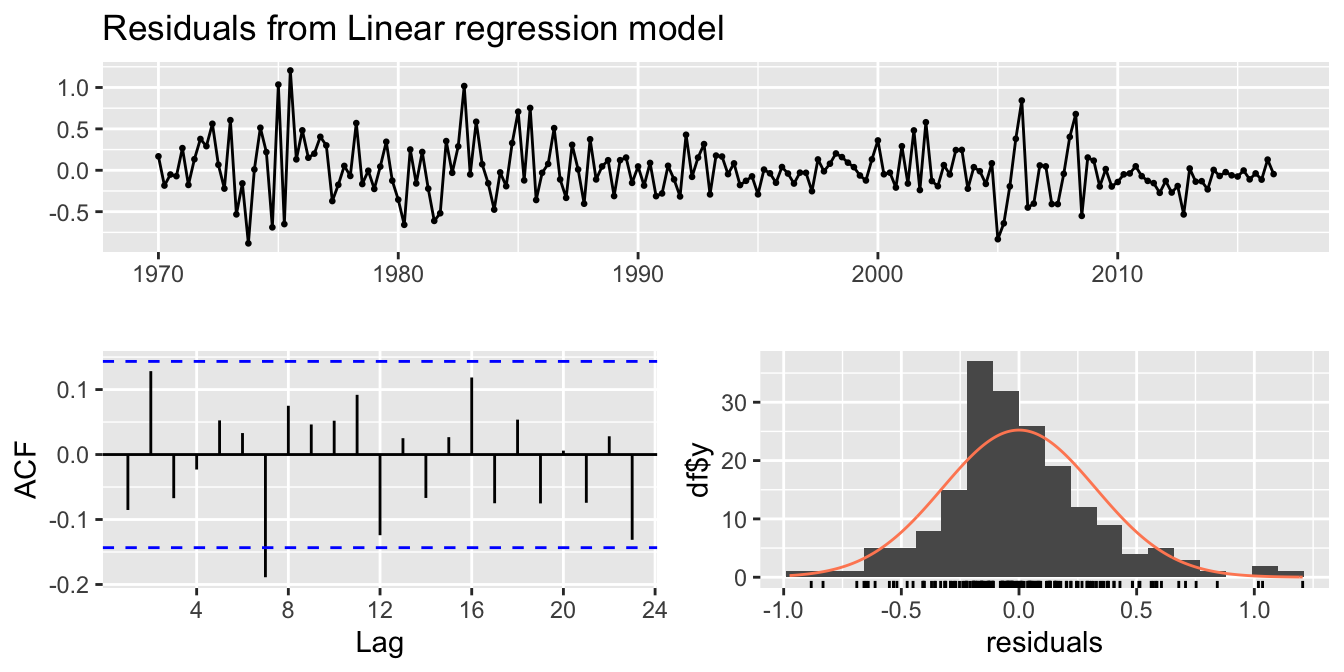
\includegraphics{The_homework_3_files/figure-latex/unnamed-chunk-3-1.pdf}

By compare the ACF and PACF graphic, we could find the AR(4) or
ARMA(4,0,0) include all the possible relationship such the residual left
with white noise (smaller than 1). Therefore we should this model for
explain the data.

3 - c

Note: I did both the mean adjust form and regression.

\begin{Shaded}
\begin{Highlighting}[]
\CommentTok{\#The following are the mean adjustment form.}

\NormalTok{mu1 }\OtherTok{\textless{}{-}} \FloatTok{0.83}
\NormalTok{mu2 }\OtherTok{\textless{}{-}} \SpecialCharTok{{-}}\FloatTok{0.34}
\NormalTok{mu3 }\OtherTok{\textless{}{-}} \FloatTok{0.55}
\NormalTok{mu4 }\OtherTok{\textless{}{-}} \SpecialCharTok{{-}}\FloatTok{0.38}
\NormalTok{c }\OtherTok{\textless{}{-}} \FloatTok{162.00}

\CommentTok{\#calcuallate the variance}
\CommentTok{\#μ = c/ 1 {-} φ1 {-} φ2 {-} φ3 {-}φ4}


\NormalTok{μ }\OtherTok{\textless{}{-}}\NormalTok{ (c)}\SpecialCharTok{/}\NormalTok{(}\DecValTok{1} \SpecialCharTok{{-}}\NormalTok{ mu1 }\SpecialCharTok{{-}}\NormalTok{ mu2 }\SpecialCharTok{{-}}\NormalTok{ mu3 }\SpecialCharTok{{-}}\NormalTok{mu4)}
\FunctionTok{print}\NormalTok{(μ)}
\end{Highlighting}
\end{Shaded}

\begin{verbatim}
## [1] 476.4706
\end{verbatim}

\begin{Shaded}
\begin{Highlighting}[]
\CommentTok{\#μ \textless{}{-} 476.4706}

\NormalTok{y1968 }\OtherTok{\textless{}{-}} \DecValTok{545}
\NormalTok{y1967 }\OtherTok{\textless{}{-}}\DecValTok{552}
\NormalTok{y1966 }\OtherTok{\textless{}{-}}\DecValTok{534}
\NormalTok{y1965 }\OtherTok{\textless{}{-}}\DecValTok{512}
\NormalTok{y1964 }\OtherTok{\textless{}{-}}\DecValTok{467}

\CommentTok{\#mean: 522}

\CommentTok{\#y1969}

\CommentTok{\#y1969 \textless{}{-} μ + (φ1\^{}q)*((Yt){-} μ) + (φ2\^{}q)*((Yt\_{-}1){-}μ) + (φ3\^{}q)*((Yt\_{-}2 ){-}μ) + (φ4\^{}q)*((Yt\_{-}3){-} μ)}

\NormalTok{y1969 }\OtherTok{\textless{}{-}}\NormalTok{ μ }\SpecialCharTok{+}\NormalTok{ mu1 }\SpecialCharTok{*}\NormalTok{ (y1968 }\SpecialCharTok{{-}}\NormalTok{ μ) }\SpecialCharTok{+}\NormalTok{ mu2 }\SpecialCharTok{*}\NormalTok{(y1967}\SpecialCharTok{{-}}\NormalTok{μ) }\SpecialCharTok{+}\NormalTok{ mu3 }\SpecialCharTok{*}\NormalTok{(y1966}\SpecialCharTok{{-}}\NormalTok{μ) }\SpecialCharTok{+}\NormalTok{ mu4 }\SpecialCharTok{*}\NormalTok{ (y1965 }\SpecialCharTok{{-}}\NormalTok{ μ)}

\CommentTok{\#print(y1969)}
\CommentTok{\#1969}
\CommentTok{\#525.81}

\CommentTok{\#1970}
\NormalTok{y1970 }\OtherTok{\textless{}{-}}\NormalTok{  μ }\SpecialCharTok{+}\NormalTok{ ((mu1)}\SpecialCharTok{\^{}}\DecValTok{2}\NormalTok{) }\SpecialCharTok{*}\NormalTok{ (y1969 }\SpecialCharTok{{-}}\NormalTok{ μ) }\SpecialCharTok{+}\NormalTok{ ((mu2)}\SpecialCharTok{\^{}}\DecValTok{2}\NormalTok{) }\SpecialCharTok{*}\NormalTok{(y1968}\SpecialCharTok{{-}}\NormalTok{ μ) }\SpecialCharTok{+}\NormalTok{ ((mu3)}\SpecialCharTok{\^{}}\DecValTok{2}\NormalTok{) }\SpecialCharTok{*}\NormalTok{(y1967}\SpecialCharTok{{-}}\NormalTok{ μ) }\SpecialCharTok{+}\NormalTok{ ((mu4)}\SpecialCharTok{\^{}}\DecValTok{2}\NormalTok{) }\SpecialCharTok{*}\NormalTok{ (y1966 }\SpecialCharTok{{-}}\NormalTok{ μ)}

\CommentTok{\#print(y1970)}
\CommentTok{\#y1970}
\CommentTok{\#549.5374}

\CommentTok{\#1971}
\NormalTok{y1971 }\OtherTok{\textless{}{-}}\NormalTok{  μ }\SpecialCharTok{+}\NormalTok{ (mu1}\SpecialCharTok{\^{}}\DecValTok{3}\NormalTok{) }\SpecialCharTok{*}\NormalTok{ (y1970 }\SpecialCharTok{{-}}\NormalTok{ μ) }\SpecialCharTok{+}\NormalTok{ (mu2}\SpecialCharTok{\^{}}\DecValTok{3}\NormalTok{) }\SpecialCharTok{*}\NormalTok{(y1969}\SpecialCharTok{{-}}\NormalTok{μ) }\SpecialCharTok{+}\NormalTok{ (mu3}\SpecialCharTok{\^{}}\DecValTok{3}\NormalTok{) }\SpecialCharTok{*}\NormalTok{(y1968}\SpecialCharTok{{-}}\NormalTok{μ) }\SpecialCharTok{+}\NormalTok{ (mu4}\SpecialCharTok{\^{}}\DecValTok{3}\NormalTok{) }\SpecialCharTok{*}\NormalTok{ (y1967 }\SpecialCharTok{{-}}\NormalTok{ μ)}

\CommentTok{\#print(y1971)}
\CommentTok{\#y1971}
\CommentTok{\#523.5671}
\end{Highlighting}
\end{Shaded}

\begin{Shaded}
\begin{Highlighting}[]
\CommentTok{\#The regression form }
\CommentTok{\#because I used the y for the adjust mean form, for the data is clear to read. I will using ry to represent the forcast generate by hte regression form.}

\NormalTok{ry1969 }\OtherTok{\textless{}{-}}\NormalTok{ c }\SpecialCharTok{+}\NormalTok{ mu1 }\SpecialCharTok{*}\NormalTok{ y1968 }\SpecialCharTok{+}\NormalTok{ mu2 }\SpecialCharTok{*}\NormalTok{y1967 }\SpecialCharTok{+}\NormalTok{ mu3}\SpecialCharTok{*}\NormalTok{ y1966 }\SpecialCharTok{+}\NormalTok{ mu4 }\SpecialCharTok{*}\NormalTok{y1965}

\CommentTok{\#print(ry1969)}
\CommentTok{\#525.81}

\NormalTok{ry1970 }\OtherTok{\textless{}{-}}\NormalTok{ c }\SpecialCharTok{+}\NormalTok{ mu1 }\SpecialCharTok{*}\NormalTok{ ry1969 }\SpecialCharTok{+}\NormalTok{ mu2 }\SpecialCharTok{*}\NormalTok{y1968 }\SpecialCharTok{+}\NormalTok{ mu3}\SpecialCharTok{*}\NormalTok{ y1967 }\SpecialCharTok{+}\NormalTok{ mu4 }\SpecialCharTok{*}\NormalTok{y1966}

\CommentTok{\#print(ry1970)}
\CommentTok{\#513.8023}


\NormalTok{ry1971 }\OtherTok{\textless{}{-}}\NormalTok{ c }\SpecialCharTok{+}\NormalTok{ mu1 }\SpecialCharTok{*}\NormalTok{ ry1970 }\SpecialCharTok{+}\NormalTok{ mu2 }\SpecialCharTok{*}\NormalTok{ry1969 }\SpecialCharTok{+}\NormalTok{ mu3}\SpecialCharTok{*}\NormalTok{ y1968}\SpecialCharTok{+}\NormalTok{ mu4 }\SpecialCharTok{*}\NormalTok{y1967}
\CommentTok{\#print(ry1971)}
\CommentTok{\#499.6705}

\NormalTok{The\_forcast\_matrix }\OtherTok{\textless{}{-}} \FunctionTok{matrix}\NormalTok{(}\AttributeTok{nrow =} \DecValTok{2}\NormalTok{, }\AttributeTok{ncol =} \DecValTok{3}\NormalTok{)}


\FunctionTok{colnames}\NormalTok{(The\_forcast\_matrix) }\OtherTok{\textless{}{-}} \FunctionTok{c}\NormalTok{(}\StringTok{"1969"}\NormalTok{, }\StringTok{"1970"}\NormalTok{, }\StringTok{"1971"}\NormalTok{)}
\FunctionTok{rownames}\NormalTok{(The\_forcast\_matrix) }\OtherTok{\textless{}{-}} \FunctionTok{c}\NormalTok{(}\StringTok{"Mean\_adjust\_form"}\NormalTok{, }\StringTok{"Regression\_form"}\NormalTok{)}

\NormalTok{The\_forcast\_matrix[}\DecValTok{1}\NormalTok{, ] }\OtherTok{\textless{}{-}}\NormalTok{ (}\FunctionTok{c}\NormalTok{(y1969, y1970, y1971))}
\NormalTok{The\_forcast\_matrix[}\DecValTok{2}\NormalTok{, ]}\OtherTok{\textless{}{-}}\NormalTok{ (}\FunctionTok{c}\NormalTok{(ry1969, ry1970, ry1971))}

\FunctionTok{print}\NormalTok{(The\_forcast\_matrix)}
\end{Highlighting}
\end{Shaded}

\begin{verbatim}
##                    1969     1970     1971
## Mean_adjust_form 525.81 549.5374 523.5671
## Regression_form  525.81 513.8023 499.6705
\end{verbatim}

3- d

\begin{Shaded}
\begin{Highlighting}[]
\NormalTok{Coal\_production}\OtherTok{\textless{}{-}} \FunctionTok{window}\NormalTok{(bicoal, }\AttributeTok{start=}\DecValTok{1920}\NormalTok{, }\AttributeTok{end=}\DecValTok{1968}\NormalTok{)}
\NormalTok{evil\_forcast }\OtherTok{\textless{}{-}} \FunctionTok{forecast}\NormalTok{(}\FunctionTok{Arima}\NormalTok{(Coal\_production, }\AttributeTok{order =} \FunctionTok{c}\NormalTok{(}\DecValTok{4}\NormalTok{, }\DecValTok{0}\NormalTok{, }\DecValTok{0}\NormalTok{)))}
\FunctionTok{print}\NormalTok{(}\FunctionTok{Arima}\NormalTok{(Coal\_production, }\AttributeTok{order =} \FunctionTok{c}\NormalTok{(}\DecValTok{4}\NormalTok{, }\DecValTok{0}\NormalTok{, }\DecValTok{0}\NormalTok{)))}
\end{Highlighting}
\end{Shaded}

\begin{verbatim}
## Series: Coal_production 
## ARIMA(4,0,0) with non-zero mean 
## 
## Coefficients:
##          ar1      ar2     ar3      ar4      mean
##       0.8334  -0.3443  0.5525  -0.3780  481.5221
## s.e.  0.1366   0.1752  0.1733   0.1414   21.0591
## 
## sigma^2 = 2795:  log likelihood = -262.05
## AIC=536.1   AICc=538.1   BIC=547.45
\end{verbatim}

\begin{Shaded}
\begin{Highlighting}[]
\NormalTok{ryd1969 }\OtherTok{\textless{}{-}}\NormalTok{ c }\SpecialCharTok{+} \FloatTok{0.8334} \SpecialCharTok{*}\NormalTok{ y1968 }\SpecialCharTok{+} \SpecialCharTok{{-}}\FloatTok{0.3443} \SpecialCharTok{*}\NormalTok{y1967 }\SpecialCharTok{+} \FloatTok{0.5525}\SpecialCharTok{*}\NormalTok{ y1966 }\SpecialCharTok{+} \SpecialCharTok{{-}}\FloatTok{0.3780} \SpecialCharTok{*}\NormalTok{y1965}
\FunctionTok{print}\NormalTok{(ryd1969)}
\end{Highlighting}
\end{Shaded}

\begin{verbatim}
## [1] 527.6484
\end{verbatim}

\begin{Shaded}
\begin{Highlighting}[]
\FunctionTok{print}\NormalTok{(evil\_forcast)}
\end{Highlighting}
\end{Shaded}

\begin{verbatim}
##      Point Forecast    Lo 80    Hi 80    Lo 95    Hi 95
## 1969       527.6291 459.8804 595.3779 424.0164 631.2419
## 1970       517.1923 429.0014 605.3832 382.3160 652.0686
## 1971       503.8051 412.4786 595.1315 364.1334 643.4768
## 1972       489.2909 390.4658 588.1160 338.1510 640.4309
## 1973       482.6041 379.6439 585.5643 325.1400 640.0682
## 1974       478.5776 375.5783 581.5770 321.0537 636.1016
## 1975       474.5657 371.4760 577.6554 316.9036 632.2278
## 1976       474.4001 371.2205 577.5796 316.6006 632.1996
## 1977       475.9463 372.5126 579.3801 317.7581 634.1346
## 1978       476.5973 372.9772 580.2174 318.1240 635.0706
\end{verbatim}

first, ARMA model will always went back to its mean in the long term.
Consider the mean different between hand forecast and over data
forecast.

second, for AR(4) model, the long term forecast always on the trend back
to its expect value. Consider the the different mu, for example mu1 hand
calculate is 0.84 but in AR(4) for all data set is 0.8334.

\#\#\#\#\#\#\#

Exercise 4

4-a

\begin{Shaded}
\begin{Highlighting}[]
\NormalTok{IBM\_stock\_price}\OtherTok{\textless{}{-}} \FunctionTok{window}\NormalTok{(ibmclose)}
\FunctionTok{summary}\NormalTok{(IBM\_stock\_price)}
\end{Highlighting}
\end{Shaded}

\begin{verbatim}
##    Min. 1st Qu.  Median    Mean 3rd Qu.    Max. 
##   306.0   387.0   494.0   478.5   549.0   603.0
\end{verbatim}

\begin{Shaded}
\begin{Highlighting}[]
\FunctionTok{var}\NormalTok{(IBM\_stock\_price)}
\end{Highlighting}
\end{Shaded}

\begin{verbatim}
## [1] 7092.88
\end{verbatim}

\begin{Shaded}
\begin{Highlighting}[]
\CommentTok{\#plot the data}
\FunctionTok{plot}\NormalTok{(IBM\_stock\_price)}
\FunctionTok{abline}\NormalTok{(}\AttributeTok{h =} \DecValTok{450}\NormalTok{, }\AttributeTok{col =} \StringTok{"red"}\NormalTok{, }\AttributeTok{lty =} \DecValTok{2}\NormalTok{, }\AttributeTok{lwd =} \DecValTok{2}\NormalTok{)}
\FunctionTok{text}\NormalTok{(}\DecValTok{1}\NormalTok{, }\DecValTok{450}\NormalTok{, }\StringTok{"The Average"}\NormalTok{, }\AttributeTok{pos =} \DecValTok{4}\NormalTok{)}
\end{Highlighting}
\end{Shaded}

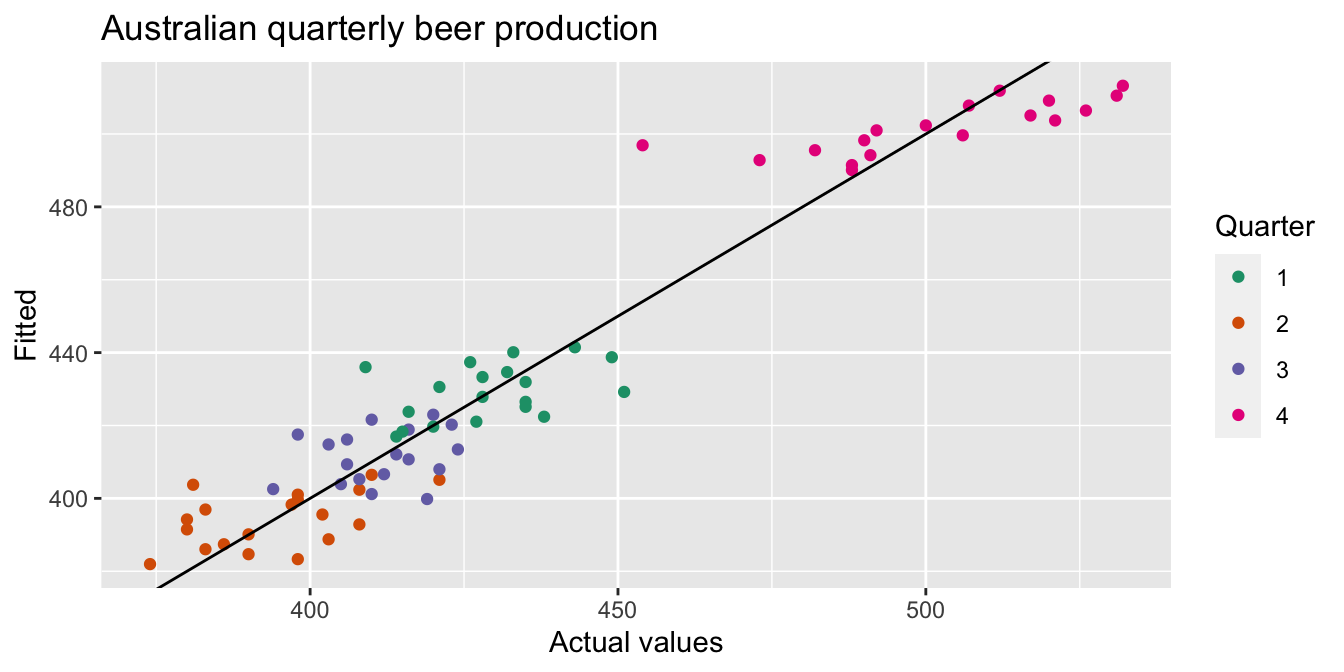
\includegraphics{The_homework_3_files/figure-latex/unnamed-chunk-8-1.pdf}

From the plot graphy, we can see a strong downward trend and a relative
big varaince, therefor the data is not stationary.

\begin{Shaded}
\begin{Highlighting}[]
\CommentTok{\#Plot the ACF and PACF}

\CommentTok{\#PACF AR SINIFICENT lag}

\FunctionTok{par}\NormalTok{(}\AttributeTok{mfrow=}\FunctionTok{c}\NormalTok{(}\DecValTok{1}\NormalTok{,}\DecValTok{2}\NormalTok{))}
\FunctionTok{Acf}\NormalTok{(IBM\_stock\_price)}
\FunctionTok{Pacf}\NormalTok{(IBM\_stock\_price)}
\end{Highlighting}
\end{Shaded}

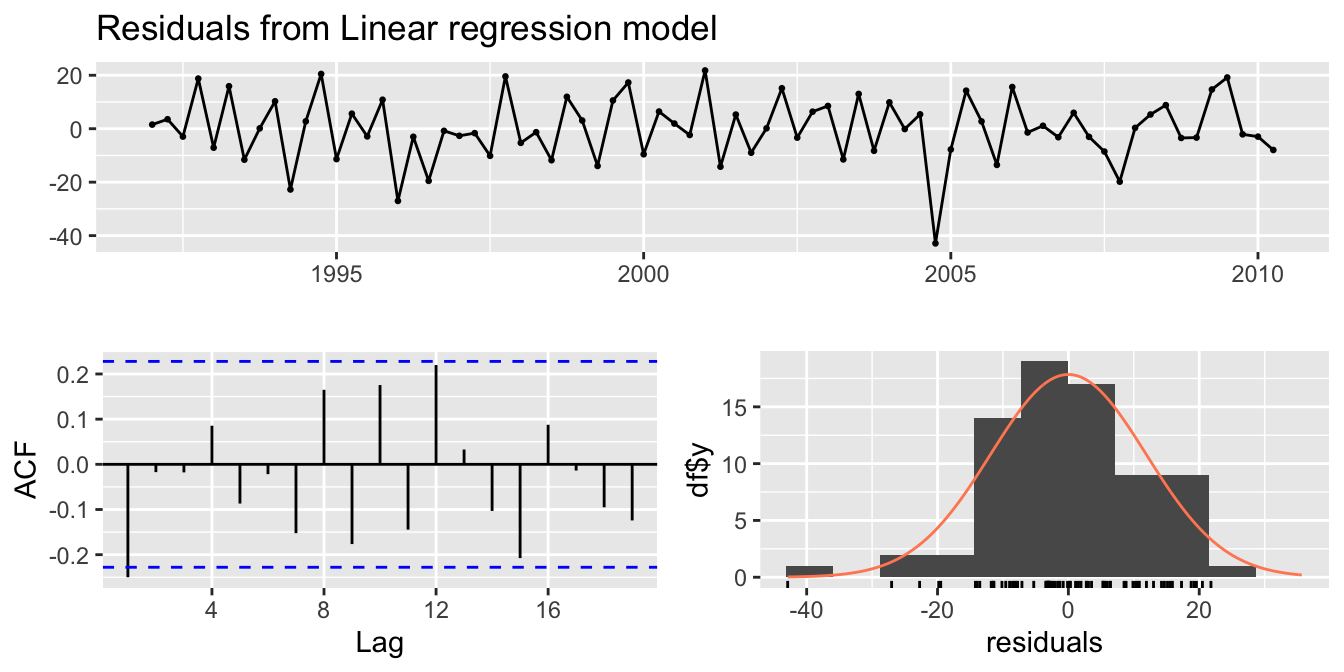
\includegraphics{The_homework_3_files/figure-latex/unnamed-chunk-9-1.pdf}

The non-stationary data ACF and PACF graphy will show the slow decaying
trend of data collection. Therefore, the IBM stock market ACF graphic
show that such data are non-stationary.

4-B

\begin{Shaded}
\begin{Highlighting}[]
\CommentTok{\#fit the model}
\NormalTok{IBM\_stock\_price\_AR\_1\_model}\OtherTok{\textless{}{-}} \FunctionTok{Arima}\NormalTok{(IBM\_stock\_price, }\AttributeTok{order =} \FunctionTok{c}\NormalTok{(}\DecValTok{1}\NormalTok{,}\DecValTok{0}\NormalTok{,}\DecValTok{0}\NormalTok{))}
\end{Highlighting}
\end{Shaded}

\begin{Shaded}
\begin{Highlighting}[]
\CommentTok{\#note: I want to try all the code that can give estimated coeffcient I knew. In case they have different reuslt and I lose the grade.}
\CommentTok{\#In the end they all give the same result.}
\FunctionTok{coef}\NormalTok{(IBM\_stock\_price\_AR\_1\_model)}
\end{Highlighting}
\end{Shaded}

\begin{verbatim}
##         ar1   intercept 
##   0.9960143 439.0382554
\end{verbatim}

\begin{Shaded}
\begin{Highlighting}[]
\FunctionTok{summary}\NormalTok{(IBM\_stock\_price\_AR\_1\_model)}
\end{Highlighting}
\end{Shaded}

\begin{verbatim}
## Series: IBM_stock_price 
## ARIMA(1,0,0) with non-zero mean 
## 
## Coefficients:
##          ar1      mean
##       0.9960  439.0383
## s.e.  0.0034   63.1365
## 
## sigma^2 = 52.77:  log likelihood = -1256.7
## AIC=2519.41   AICc=2519.47   BIC=2531.14
## 
## Training set error measures:
##                      ME     RMSE      MAE         MPE     MAPE     MASE
## Training set -0.1160196 7.244261 5.224116 -0.06302297 1.199337 1.002856
##                    ACF1
## Training set 0.09004763
\end{verbatim}

\begin{Shaded}
\begin{Highlighting}[]
\NormalTok{(fit2 }\OtherTok{\textless{}{-}} \FunctionTok{Arima}\NormalTok{(IBM\_stock\_price, }\AttributeTok{order =} \FunctionTok{c}\NormalTok{(}\DecValTok{1}\NormalTok{,}\DecValTok{0}\NormalTok{,}\DecValTok{0}\NormalTok{)))}
\end{Highlighting}
\end{Shaded}

\begin{verbatim}
## Series: IBM_stock_price 
## ARIMA(1,0,0) with non-zero mean 
## 
## Coefficients:
##          ar1      mean
##       0.9960  439.0383
## s.e.  0.0034   63.1365
## 
## sigma^2 = 52.77:  log likelihood = -1256.7
## AIC=2519.41   AICc=2519.47   BIC=2531.14
\end{verbatim}

The estimated coefficient measures the correlation between one
observation and the previous observation. It indicates the correlation
relationship between two observations, where a positive coefficient
signifies a positive relationship and a negative coefficient signifies a
negative relationship. the larger the number, the stronger the
relationship. In this case, it means the data has a strong positive
correlation relationship representing the data is not fully stationary
enough.

4-c

\begin{Shaded}
\begin{Highlighting}[]
\CommentTok{\#Use R to plot the first difference of the series, the ACF and PACF. Explain how each plot shows that the differenced series is stationary.}

\NormalTok{IBM\_stock\_price\_difference }\OtherTok{\textless{}{-}} \FunctionTok{diff}\NormalTok{(IBM\_stock\_price, }\AttributeTok{lag =} \DecValTok{1}\NormalTok{)}

\FunctionTok{summary}\NormalTok{(IBM\_stock\_price\_difference)}
\end{Highlighting}
\end{Shaded}

\begin{verbatim}
##     Min.  1st Qu.   Median     Mean  3rd Qu.     Max. 
## -38.0000  -4.0000   0.0000  -0.2799   4.0000  27.0000
\end{verbatim}

\begin{Shaded}
\begin{Highlighting}[]
\FunctionTok{plot}\NormalTok{(IBM\_stock\_price\_difference)}
\FunctionTok{abline}\NormalTok{(}\AttributeTok{h =} \SpecialCharTok{{-}}\FloatTok{0.2799}\NormalTok{, }\AttributeTok{col =} \StringTok{"red"}\NormalTok{, }\AttributeTok{lty =} \DecValTok{2}\NormalTok{, }\AttributeTok{lwd =} \DecValTok{2}\NormalTok{)}
\FunctionTok{text}\NormalTok{(}\DecValTok{1}\NormalTok{, }\SpecialCharTok{{-}}\DecValTok{10}\NormalTok{, }\StringTok{"The Average"}\NormalTok{, }\AttributeTok{pos =} \DecValTok{4}\NormalTok{)}
\end{Highlighting}
\end{Shaded}

\includegraphics{The_homework_3_files/figure-latex/unnamed-chunk-12-1.pdf}

The plot does not display any visible trend and moving around the
average compare the un-stationary verson.

\begin{Shaded}
\begin{Highlighting}[]
\FunctionTok{par}\NormalTok{(}\AttributeTok{mfrow=}\FunctionTok{c}\NormalTok{(}\DecValTok{1}\NormalTok{,}\DecValTok{2}\NormalTok{))}
\FunctionTok{Acf}\NormalTok{(IBM\_stock\_price\_difference)}
\FunctionTok{Pacf}\NormalTok{(IBM\_stock\_price\_difference)}
\end{Highlighting}
\end{Shaded}

\includegraphics{The_homework_3_files/figure-latex/unnamed-chunk-13-1.pdf}

The ACF and PACF graphic does not show the slow decaying trend means
that the observation have little or non relationship (correlation) with
each others compare to the non-stationary data.

4-d

\begin{Shaded}
\begin{Highlighting}[]
\NormalTok{IBM\_stock\_price\_AR\_1\_model\_differencedata}\OtherTok{\textless{}{-}} \FunctionTok{Arima}\NormalTok{(IBM\_stock\_price\_difference, }\AttributeTok{order =} \FunctionTok{c}\NormalTok{(}\DecValTok{1}\NormalTok{,}\DecValTok{0}\NormalTok{,}\DecValTok{0}\NormalTok{))}

\CommentTok{\#since all three way will give the same estimated coeffcient, so I will use summary()}

\FunctionTok{summary}\NormalTok{(IBM\_stock\_price\_AR\_1\_model\_differencedata)}
\end{Highlighting}
\end{Shaded}

\begin{verbatim}
## Series: IBM_stock_price_difference 
## ARIMA(1,0,0) with non-zero mean 
## 
## Coefficients:
##          ar1     mean
##       0.0855  -0.2792
## s.e.  0.0519   0.4115
## 
## sigma^2 = 52.44:  log likelihood = -1249.74
## AIC=2505.49   AICc=2505.55   BIC=2517.21
## 
## Training set error measures:
##                        ME     RMSE      MAE MPE MAPE      MASE         ACF1
## Training set 0.0006553438 7.221707 5.219951 NaN  Inf 0.7471614 0.0009409713
\end{verbatim}

The estimated coefficient is 0.0855 which is smaller than 0.9960 in the
question 4-c.~by different the data, the correlation relationship
between observation have been massively decreased. In other word, the
data been stationary,

\#\#\#\#

Exercise 5

5-a

\begin{Shaded}
\begin{Highlighting}[]
\NormalTok{GGDP\_raw }\OtherTok{\textless{}{-}} \FunctionTok{read\_csv}\NormalTok{(}\StringTok{"/Users/tie/SynologyDrive/nn/ECON{-}493{-}forcasting{-}economy/493 homework/homework 3/NAEXKP01CAQ661S.csv"}\NormalTok{, }\AttributeTok{col\_types =} \FunctionTok{cols}\NormalTok{(}\AttributeTok{NAEXKP01CAQ661S =} \FunctionTok{col\_number}\NormalTok{()))}

\FunctionTok{plot}\NormalTok{(GGDP\_raw, }\AttributeTok{type =} \StringTok{"l"}\NormalTok{)}
\FunctionTok{abline}\NormalTok{(}\AttributeTok{h =} \FloatTok{64.35}\NormalTok{, }\AttributeTok{col =} \StringTok{"red"}\NormalTok{, }\AttributeTok{lty =} \DecValTok{2}\NormalTok{, }\AttributeTok{lwd =} \DecValTok{2}\NormalTok{)}
\FunctionTok{text}\NormalTok{(}\DecValTok{1}\NormalTok{, }\DecValTok{60}\NormalTok{, }\StringTok{"The Average"}\NormalTok{, }\AttributeTok{pos =} \DecValTok{4}\NormalTok{)}
\end{Highlighting}
\end{Shaded}

\includegraphics{The_homework_3_files/figure-latex/unnamed-chunk-15-1.pdf}

The plot data show the upward trend, therefore the data need to be
stationary.

\begin{Shaded}
\begin{Highlighting}[]
\FunctionTok{par}\NormalTok{(}\AttributeTok{mfrow=}\FunctionTok{c}\NormalTok{(}\DecValTok{1}\NormalTok{,}\DecValTok{2}\NormalTok{))}
\FunctionTok{Acf}\NormalTok{(GGDP\_raw}\SpecialCharTok{$}\NormalTok{NAEXKP01CAQ661S)}
\FunctionTok{Pacf}\NormalTok{(GGDP\_raw}\SpecialCharTok{$}\NormalTok{NAEXKP01CAQ661S)}
\end{Highlighting}
\end{Shaded}

\includegraphics{The_homework_3_files/figure-latex/unnamed-chunk-16-1.pdf}

\begin{Shaded}
\begin{Highlighting}[]
\NormalTok{GGDP }\OtherTok{\textless{}{-}}\NormalTok{ GGDP\_raw}
\end{Highlighting}
\end{Shaded}

The non-stationary data ACF and PACF graphs will show a slow downward
trend. In this data set, the ACF graph shows a slow downward trend,
therefore, thus GDP data need to be stationary.

5-b

\begin{Shaded}
\begin{Highlighting}[]
\CommentTok{\#Use R to plot the change in log RGDP}

\NormalTok{log\_different\_GGPD }\OtherTok{\textless{}{-}} \FunctionTok{diff}\NormalTok{(}\FunctionTok{log}\NormalTok{(GGDP}\SpecialCharTok{$}\NormalTok{NAEXKP01CAQ661S), }\AttributeTok{lag =} \DecValTok{1}\NormalTok{)}
\FunctionTok{summary}\NormalTok{(log\_different\_GGPD)}
\end{Highlighting}
\end{Shaded}

\begin{verbatim}
##      Min.   1st Qu.    Median      Mean   3rd Qu.      Max. 
## -0.023114  0.003273  0.007256  0.007815  0.012877  0.030930
\end{verbatim}

\begin{Shaded}
\begin{Highlighting}[]
\FunctionTok{plot}\NormalTok{(log\_different\_GGPD, }\AttributeTok{type =} \StringTok{"l"}\NormalTok{)}
\end{Highlighting}
\end{Shaded}

\includegraphics{The_homework_3_files/figure-latex/unnamed-chunk-17-1.pdf}

The plot graph still have a down turn, which may suggest it is not fully
stationary.

\begin{Shaded}
\begin{Highlighting}[]
\FunctionTok{par}\NormalTok{(}\AttributeTok{mfrow=}\FunctionTok{c}\NormalTok{(}\DecValTok{1}\NormalTok{,}\DecValTok{2}\NormalTok{))}
\FunctionTok{Acf}\NormalTok{(log\_different\_GGPD)}
\FunctionTok{Pacf}\NormalTok{(log\_different\_GGPD)}
\end{Highlighting}
\end{Shaded}

\includegraphics{The_homework_3_files/figure-latex/unnamed-chunk-18-1.pdf}

The ACF graphy suggest the same things. even there is a fast drop but
the are slow and constant drop.

5-c

The ACF and PACF graph suggest both AR() and MA() (AKA: ARMA) because
both graph display significant spikes.

3 lag in the ACF so its need to be MA(4)

3 lag in the PACF so its need to be AR(4)

ARMA (4, 0 ,4)

\begin{Shaded}
\begin{Highlighting}[]
\CommentTok{\#by using the function auto\_arima() we cound just find the answer...}
\NormalTok{test\_one }\OtherTok{\textless{}{-}} \FunctionTok{auto.arima}\NormalTok{(log\_different\_GGPD)}
\FunctionTok{print}\NormalTok{(test\_one)}
\end{Highlighting}
\end{Shaded}

\begin{verbatim}
## Series: log_different_GGPD 
## ARIMA(2,1,1) 
## 
## Coefficients:
##          ar1     ar2      ma1
##       0.2947  0.0450  -0.9615
## s.e.  0.0691  0.0686   0.0207
## 
## sigma^2 = 6.165e-05:  log likelihood = 778.73
## AIC=-1549.45   AICc=-1549.27   BIC=-1535.75
\end{verbatim}

\begin{Shaded}
\begin{Highlighting}[]
\CommentTok{\#This is a loop test from ARMA(1,1,0) to ARMA(10, 1, 0). choise 10 beacase the answer is 4 (see code in 3{-}c)}

\NormalTok{BIC\_test }\OtherTok{\textless{}{-}} \FunctionTok{matrix}\NormalTok{(}\DecValTok{0}\NormalTok{, }\AttributeTok{nrow =} \DecValTok{10}\NormalTok{, }\AttributeTok{ncol =} \DecValTok{2}\NormalTok{)}

\ControlFlowTok{for}\NormalTok{(i }\ControlFlowTok{in} \DecValTok{1}\SpecialCharTok{:}\DecValTok{10}\NormalTok{)\{BIC\_test[i,}\DecValTok{1}\NormalTok{] }\OtherTok{\textless{}{-}}\NormalTok{ i\}}

\NormalTok{BIC\_test[}\DecValTok{1}\NormalTok{,}\DecValTok{2}\NormalTok{] }\OtherTok{\textless{}{-}} \FunctionTok{BIC}\NormalTok{(}\FunctionTok{Arima}\NormalTok{(log\_different\_GGPD, }\AttributeTok{order =} \FunctionTok{c}\NormalTok{(}\DecValTok{1}\NormalTok{,}\DecValTok{0}\NormalTok{,}\DecValTok{0}\NormalTok{), }\AttributeTok{include.drift =} \ConstantTok{TRUE}\NormalTok{))}
\NormalTok{BIC\_test[}\DecValTok{2}\NormalTok{,}\DecValTok{2}\NormalTok{] }\OtherTok{\textless{}{-}} \FunctionTok{BIC}\NormalTok{(}\FunctionTok{Arima}\NormalTok{(log\_different\_GGPD, }\AttributeTok{order =} \FunctionTok{c}\NormalTok{(}\DecValTok{2}\NormalTok{,}\DecValTok{0}\NormalTok{,}\DecValTok{0}\NormalTok{), }\AttributeTok{include.drift =} \ConstantTok{TRUE}\NormalTok{))}
\NormalTok{BIC\_test[}\DecValTok{3}\NormalTok{,}\DecValTok{2}\NormalTok{] }\OtherTok{\textless{}{-}} \FunctionTok{BIC}\NormalTok{(}\FunctionTok{Arima}\NormalTok{(log\_different\_GGPD, }\AttributeTok{order =} \FunctionTok{c}\NormalTok{(}\DecValTok{3}\NormalTok{,}\DecValTok{0}\NormalTok{,}\DecValTok{0}\NormalTok{), }\AttributeTok{include.drift =} \ConstantTok{TRUE}\NormalTok{))}
\NormalTok{BIC\_test[}\DecValTok{4}\NormalTok{,}\DecValTok{2}\NormalTok{] }\OtherTok{\textless{}{-}} \FunctionTok{BIC}\NormalTok{(}\FunctionTok{Arima}\NormalTok{(log\_different\_GGPD, }\AttributeTok{order =} \FunctionTok{c}\NormalTok{(}\DecValTok{4}\NormalTok{,}\DecValTok{0}\NormalTok{,}\DecValTok{0}\NormalTok{), }\AttributeTok{include.drift =} \ConstantTok{TRUE}\NormalTok{))}
\NormalTok{BIC\_test[}\DecValTok{5}\NormalTok{,}\DecValTok{2}\NormalTok{] }\OtherTok{\textless{}{-}} \FunctionTok{BIC}\NormalTok{(}\FunctionTok{Arima}\NormalTok{(log\_different\_GGPD, }\AttributeTok{order =} \FunctionTok{c}\NormalTok{(}\DecValTok{5}\NormalTok{,}\DecValTok{0}\NormalTok{,}\DecValTok{0}\NormalTok{), }\AttributeTok{include.drift =} \ConstantTok{TRUE}\NormalTok{))}
\NormalTok{BIC\_test[}\DecValTok{6}\NormalTok{,}\DecValTok{2}\NormalTok{] }\OtherTok{\textless{}{-}} \FunctionTok{BIC}\NormalTok{(}\FunctionTok{Arima}\NormalTok{(log\_different\_GGPD, }\AttributeTok{order =} \FunctionTok{c}\NormalTok{(}\DecValTok{6}\NormalTok{,}\DecValTok{0}\NormalTok{,}\DecValTok{0}\NormalTok{), }\AttributeTok{include.drift =} \ConstantTok{TRUE}\NormalTok{))}
\NormalTok{BIC\_test[}\DecValTok{7}\NormalTok{,}\DecValTok{2}\NormalTok{] }\OtherTok{\textless{}{-}} \FunctionTok{BIC}\NormalTok{(}\FunctionTok{Arima}\NormalTok{(log\_different\_GGPD, }\AttributeTok{order =} \FunctionTok{c}\NormalTok{(}\DecValTok{7}\NormalTok{,}\DecValTok{0}\NormalTok{,}\DecValTok{0}\NormalTok{), }\AttributeTok{include.drift =} \ConstantTok{TRUE}\NormalTok{))}
\NormalTok{BIC\_test[}\DecValTok{8}\NormalTok{,}\DecValTok{2}\NormalTok{] }\OtherTok{\textless{}{-}} \FunctionTok{BIC}\NormalTok{(}\FunctionTok{Arima}\NormalTok{(log\_different\_GGPD, }\AttributeTok{order =} \FunctionTok{c}\NormalTok{(}\DecValTok{8}\NormalTok{,}\DecValTok{0}\NormalTok{,}\DecValTok{0}\NormalTok{), }\AttributeTok{include.drift =} \ConstantTok{TRUE}\NormalTok{))}
\NormalTok{BIC\_test[}\DecValTok{9}\NormalTok{,}\DecValTok{2}\NormalTok{] }\OtherTok{\textless{}{-}} \FunctionTok{BIC}\NormalTok{(}\FunctionTok{Arima}\NormalTok{(log\_different\_GGPD, }\AttributeTok{order =} \FunctionTok{c}\NormalTok{(}\DecValTok{9}\NormalTok{,}\DecValTok{0}\NormalTok{,}\DecValTok{0}\NormalTok{), }\AttributeTok{include.drift =} \ConstantTok{TRUE}\NormalTok{))}
\NormalTok{BIC\_test[}\DecValTok{10}\NormalTok{,}\DecValTok{2}\NormalTok{] }\OtherTok{\textless{}{-}} \FunctionTok{BIC}\NormalTok{(}\FunctionTok{Arima}\NormalTok{(log\_different\_GGPD, }\AttributeTok{order =} \FunctionTok{c}\NormalTok{(}\DecValTok{10}\NormalTok{,}\DecValTok{0}\NormalTok{,}\DecValTok{0}\NormalTok{), }\AttributeTok{include.drift =} \ConstantTok{TRUE}\NormalTok{))}


\FunctionTok{print}\NormalTok{(BIC\_test)}
\end{Highlighting}
\end{Shaded}

\begin{verbatim}
##       [,1]      [,2]
##  [1,]    1 -1551.448
##  [2,]    2 -1546.548
##  [3,]    3 -1541.287
##  [4,]    4 -1535.858
##  [5,]    5 -1531.438
##  [6,]    6 -1526.010
##  [7,]    7 -1520.622
##  [8,]    8 -1517.440
##  [9,]    9 -1515.869
## [10,]   10 -1510.502
\end{verbatim}

According to the BIC test Matrix, the AR(1) has the lowest absolute BIC,
therefore it is the best for AR(1) for describe model.

3-e

\begin{Shaded}
\begin{Highlighting}[]
\NormalTok{AIC\_test }\OtherTok{\textless{}{-}} \FunctionTok{matrix}\NormalTok{(}\DecValTok{0}\NormalTok{, }\AttributeTok{nrow =} \DecValTok{10}\NormalTok{, }\AttributeTok{ncol =} \DecValTok{2}\NormalTok{)}

\ControlFlowTok{for}\NormalTok{(i }\ControlFlowTok{in} \DecValTok{1}\SpecialCharTok{:}\DecValTok{10}\NormalTok{)\{AIC\_test[i,}\DecValTok{1}\NormalTok{] }\OtherTok{\textless{}{-}}\NormalTok{ i\}}

\NormalTok{AIC\_test[}\DecValTok{1}\NormalTok{,}\DecValTok{2}\NormalTok{] }\OtherTok{\textless{}{-}} \FunctionTok{AIC}\NormalTok{(}\FunctionTok{Arima}\NormalTok{(log\_different\_GGPD, }\AttributeTok{order =} \FunctionTok{c}\NormalTok{(}\DecValTok{1}\NormalTok{,}\DecValTok{0}\NormalTok{,}\DecValTok{0}\NormalTok{), }\AttributeTok{include.drift =} \ConstantTok{TRUE}\NormalTok{))}
\NormalTok{AIC\_test[}\DecValTok{2}\NormalTok{,}\DecValTok{2}\NormalTok{] }\OtherTok{\textless{}{-}} \FunctionTok{AIC}\NormalTok{(}\FunctionTok{Arima}\NormalTok{(log\_different\_GGPD, }\AttributeTok{order =} \FunctionTok{c}\NormalTok{(}\DecValTok{2}\NormalTok{,}\DecValTok{0}\NormalTok{,}\DecValTok{0}\NormalTok{), }\AttributeTok{include.drift =} \ConstantTok{TRUE}\NormalTok{))}
\NormalTok{AIC\_test[}\DecValTok{3}\NormalTok{,}\DecValTok{2}\NormalTok{] }\OtherTok{\textless{}{-}} \FunctionTok{AIC}\NormalTok{(}\FunctionTok{Arima}\NormalTok{(log\_different\_GGPD, }\AttributeTok{order =} \FunctionTok{c}\NormalTok{(}\DecValTok{3}\NormalTok{,}\DecValTok{0}\NormalTok{,}\DecValTok{0}\NormalTok{), }\AttributeTok{include.drift =} \ConstantTok{TRUE}\NormalTok{))}
\NormalTok{AIC\_test[}\DecValTok{4}\NormalTok{,}\DecValTok{2}\NormalTok{] }\OtherTok{\textless{}{-}} \FunctionTok{AIC}\NormalTok{(}\FunctionTok{Arima}\NormalTok{(log\_different\_GGPD, }\AttributeTok{order =} \FunctionTok{c}\NormalTok{(}\DecValTok{4}\NormalTok{,}\DecValTok{0}\NormalTok{,}\DecValTok{0}\NormalTok{), }\AttributeTok{include.drift =} \ConstantTok{TRUE}\NormalTok{))}
\NormalTok{AIC\_test[}\DecValTok{5}\NormalTok{,}\DecValTok{2}\NormalTok{] }\OtherTok{\textless{}{-}} \FunctionTok{AIC}\NormalTok{(}\FunctionTok{Arima}\NormalTok{(log\_different\_GGPD, }\AttributeTok{order =} \FunctionTok{c}\NormalTok{(}\DecValTok{5}\NormalTok{,}\DecValTok{0}\NormalTok{,}\DecValTok{0}\NormalTok{), }\AttributeTok{include.drift =} \ConstantTok{TRUE}\NormalTok{))}
\NormalTok{AIC\_test[}\DecValTok{6}\NormalTok{,}\DecValTok{2}\NormalTok{] }\OtherTok{\textless{}{-}} \FunctionTok{AIC}\NormalTok{(}\FunctionTok{Arima}\NormalTok{(log\_different\_GGPD, }\AttributeTok{order =} \FunctionTok{c}\NormalTok{(}\DecValTok{6}\NormalTok{,}\DecValTok{0}\NormalTok{,}\DecValTok{0}\NormalTok{), }\AttributeTok{include.drift =} \ConstantTok{TRUE}\NormalTok{))}
\NormalTok{AIC\_test[}\DecValTok{7}\NormalTok{,}\DecValTok{2}\NormalTok{] }\OtherTok{\textless{}{-}} \FunctionTok{AIC}\NormalTok{(}\FunctionTok{Arima}\NormalTok{(log\_different\_GGPD, }\AttributeTok{order =} \FunctionTok{c}\NormalTok{(}\DecValTok{7}\NormalTok{,}\DecValTok{0}\NormalTok{,}\DecValTok{0}\NormalTok{), }\AttributeTok{include.drift =} \ConstantTok{TRUE}\NormalTok{))}
\NormalTok{AIC\_test[}\DecValTok{8}\NormalTok{,}\DecValTok{2}\NormalTok{] }\OtherTok{\textless{}{-}} \FunctionTok{AIC}\NormalTok{(}\FunctionTok{Arima}\NormalTok{(log\_different\_GGPD, }\AttributeTok{order =} \FunctionTok{c}\NormalTok{(}\DecValTok{8}\NormalTok{,}\DecValTok{0}\NormalTok{,}\DecValTok{0}\NormalTok{), }\AttributeTok{include.drift =} \ConstantTok{TRUE}\NormalTok{))}
\NormalTok{AIC\_test[}\DecValTok{9}\NormalTok{,}\DecValTok{2}\NormalTok{] }\OtherTok{\textless{}{-}} \FunctionTok{AIC}\NormalTok{(}\FunctionTok{Arima}\NormalTok{(log\_different\_GGPD, }\AttributeTok{order =} \FunctionTok{c}\NormalTok{(}\DecValTok{9}\NormalTok{,}\DecValTok{0}\NormalTok{,}\DecValTok{0}\NormalTok{), }\AttributeTok{include.drift =} \ConstantTok{TRUE}\NormalTok{))}
\NormalTok{AIC\_test[}\DecValTok{10}\NormalTok{,}\DecValTok{2}\NormalTok{] }\OtherTok{\textless{}{-}} \FunctionTok{AIC}\NormalTok{(}\FunctionTok{Arima}\NormalTok{(log\_different\_GGPD, }\AttributeTok{order =} \FunctionTok{c}\NormalTok{(}\DecValTok{10}\NormalTok{,}\DecValTok{0}\NormalTok{,}\DecValTok{0}\NormalTok{), }\AttributeTok{include.drift =} \ConstantTok{TRUE}\NormalTok{))}

                      
\FunctionTok{print}\NormalTok{(AIC\_test)}
\end{Highlighting}
\end{Shaded}

\begin{verbatim}
##       [,1]      [,2]
##  [1,]    1 -1565.165
##  [2,]    2 -1563.695
##  [3,]    3 -1561.863
##  [4,]    4 -1559.863
##  [5,]    5 -1558.873
##  [6,]    6 -1556.874
##  [7,]    7 -1554.916
##  [8,]    8 -1555.163
##  [9,]    9 -1557.021
## [10,]   10 -1555.084
\end{verbatim}

According to AIC test matrix, the AR(1) has the lowest absolute value,
therefore, according to AIC test, Ar(1) is THE best adequately describe
the chagne in log RGDP.

\hypertarget{section}{%
\subsubsection{}\label{section}}

\begin{enumerate}
\def\labelenumi{\alph{enumi}.}
\setcounter{enumi}{5}
\tightlist
\item
  Use the models selected in parts (d) and (e) to forecast the quarterly
  log RGDP in 2018:Q2, 2018:Q3, and 2018:Q4. Compare your results.
\end{enumerate}

AIC and BIC test show that AR(1) is the best model.

\begin{Shaded}
\begin{Highlighting}[]
\NormalTok{Q5\_f\_d }\OtherTok{\textless{}{-}} \FunctionTok{forecast}\NormalTok{(}\FunctionTok{Arima}\NormalTok{(}\FunctionTok{diff}\NormalTok{(}\FunctionTok{log}\NormalTok{(GGDP}\SpecialCharTok{$}\NormalTok{NAEXKP01CAQ661S), }\AttributeTok{lag =} \DecValTok{4}\NormalTok{), }\AttributeTok{order =} \FunctionTok{c}\NormalTok{(}\DecValTok{1}\NormalTok{, }\DecValTok{0}\NormalTok{, }\DecValTok{0}\NormalTok{), }\AttributeTok{include.drift =} \ConstantTok{TRUE}\NormalTok{))}

\FunctionTok{print}\NormalTok{(Q5\_f\_d)}
\end{Highlighting}
\end{Shaded}

\begin{verbatim}
##     Point Forecast        Lo 80      Hi 80         Lo 95      Hi 95
## 226     0.02116382  0.007187593 0.03514005 -0.0002109758 0.04253862
## 227     0.01973173  0.001326942 0.03813651 -0.0084159634 0.04787942
## 228     0.01847955 -0.002592020 0.03955113 -0.0137466361 0.05070574
## 229     0.01738153 -0.005450387 0.04021346 -0.0175368755 0.05229994
## 230     0.01641560 -0.007626740 0.04045794 -0.0203539865 0.05318519
## 231     0.01556284 -0.009330672 0.04045635 -0.0225084998 0.05363418
## 232     0.01480704 -0.010693257 0.04030734 -0.0241923006 0.05380638
## 233     0.01413433 -0.011802398 0.04007106 -0.0255324723 0.05380113
## 234     0.01353280 -0.012719702 0.03978531 -0.0266169378 0.05368254
## 235     0.01299227 -0.013489660 0.03947420 -0.0275083454 0.05349288
\end{verbatim}

2018:Q2 0.02116382 0.007187593 0.03514005 -0.0002109758 0.04253862 c

2018:Q3 0.01973173 0.001326942 0.03813651 -0.0084159634 0.04787942

2018:Q4 0.01847955 -0.002592020 0.03955113 -0.0137466361 0.05070574

According to AIC test matrix, the AR(2) has the lowest absolute value,
therefore, according to AIC test, AT(2) is THE best adequately describe
the chagne in log RGDP.

(I love Coding, and coding make me happy!)

\end{document}
